\setcounter{chapter}{6}
\chapter{Planar Graphs}
\makeheading{2020-03-23}
\section{Planarity}
$ K_4 $ is the complete graph on $ 4 $ vertices.
There are $ \binom{4}{2}=6 $ edges.

\tikzset{every picture/.style={line width=0.75pt}} %set default line width to 0.75pt        

\begin{center}
    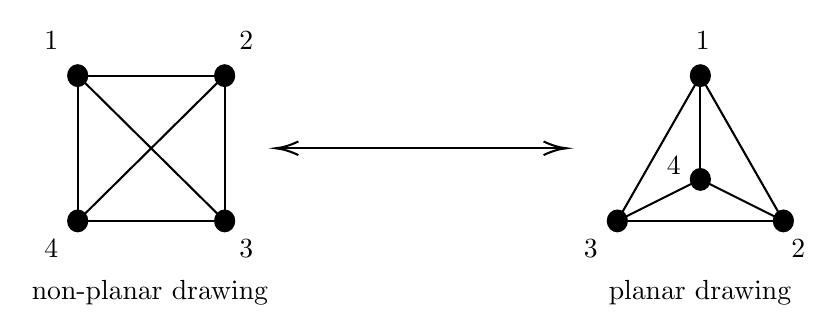
\begin{tikzpicture}[x=0.75pt,y=0.75pt,yscale=-1,xscale=1]
        %uncomment if require: \path (0,474); %set diagram left start at 0, and has height of 474

        %Flowchart: Connector [id:dp3510867786055979] 
        \draw  [fill={rgb, 255:red, 0; green, 0; blue, 0 }  ,fill opacity=1 ] (190.8,45) .. controls (190.8,42.24) and (192.86,40) .. (195.4,40) .. controls (197.94,40) and (200,42.24) .. (200,45) .. controls (200,47.76) and (197.94,50) .. (195.4,50) .. controls (192.86,50) and (190.8,47.76) .. (190.8,45) -- cycle ;
        %Flowchart: Connector [id:dp23325011502371185] 
        \draw  [fill={rgb, 255:red, 0; green, 0; blue, 0 }  ,fill opacity=1 ] (120,45) .. controls (120,42.24) and (122.06,40) .. (124.6,40) .. controls (127.14,40) and (129.2,42.24) .. (129.2,45) .. controls (129.2,47.76) and (127.14,50) .. (124.6,50) .. controls (122.06,50) and (120,47.76) .. (120,45) -- cycle ;
        %Flowchart: Connector [id:dp23142334311701362] 
        \draw  [fill={rgb, 255:red, 0; green, 0; blue, 0 }  ,fill opacity=1 ] (120,115) .. controls (120,112.24) and (122.06,110) .. (124.6,110) .. controls (127.14,110) and (129.2,112.24) .. (129.2,115) .. controls (129.2,117.76) and (127.14,120) .. (124.6,120) .. controls (122.06,120) and (120,117.76) .. (120,115) -- cycle ;
        %Flowchart: Connector [id:dp7797455570779843] 
        \draw  [fill={rgb, 255:red, 0; green, 0; blue, 0 }  ,fill opacity=1 ] (190.8,115) .. controls (190.8,112.24) and (192.86,110) .. (195.4,110) .. controls (197.94,110) and (200,112.24) .. (200,115) .. controls (200,117.76) and (197.94,120) .. (195.4,120) .. controls (192.86,120) and (190.8,117.76) .. (190.8,115) -- cycle ;
        %Straight Lines [id:da41532672128108983] 
        \draw    (124.6,45) -- (195.4,45) ;
        %Straight Lines [id:da5760893830670054] 
        \draw    (124.6,115) -- (195.4,115) ;
        %Straight Lines [id:da9817133471375197] 
        \draw    (124.6,45) -- (124.6,115) ;
        %Straight Lines [id:da4535563591277284] 
        \draw    (195.4,45) -- (195.4,115) ;
        %Straight Lines [id:da1716138690236103] 
        \draw    (124.6,45) -- (195.4,115) ;
        %Straight Lines [id:da2193825139965403] 
        \draw    (195.4,45) -- (124.6,115) ;

        %Straight Lines [id:da07684673490154237] 
        \draw    (220,80) -- (358,80) ;
        \draw [shift={(360,80)}, rotate = 180] [color={rgb, 255:red, 0; green, 0; blue, 0 }  ][line width=0.75]    (10.93,-3.29) .. controls (6.95,-1.4) and (3.31,-0.3) .. (0,0) .. controls (3.31,0.3) and (6.95,1.4) .. (10.93,3.29)   ;
        %Straight Lines [id:da07839548506909066] 
        \draw    (360,80) -- (222,80) ;
        \draw [shift={(220,80)}, rotate = 360] [color={rgb, 255:red, 0; green, 0; blue, 0 }  ][line width=0.75]    (10.93,-3.29) .. controls (6.95,-1.4) and (3.31,-0.3) .. (0,0) .. controls (3.31,0.3) and (6.95,1.4) .. (10.93,3.29)   ;
        %Flowchart: Connector [id:dp5067832375402825] 
        \draw  [fill={rgb, 255:red, 0; green, 0; blue, 0 }  ,fill opacity=1 ] (420,45) .. controls (420,42.24) and (422.06,40) .. (424.6,40) .. controls (427.14,40) and (429.2,42.24) .. (429.2,45) .. controls (429.2,47.76) and (427.14,50) .. (424.6,50) .. controls (422.06,50) and (420,47.76) .. (420,45) -- cycle ;
        %Flowchart: Connector [id:dp6010818659882411] 
        \draw  [fill={rgb, 255:red, 0; green, 0; blue, 0 }  ,fill opacity=1 ] (420,95) .. controls (420,92.24) and (422.06,90) .. (424.6,90) .. controls (427.14,90) and (429.2,92.24) .. (429.2,95) .. controls (429.2,97.76) and (427.14,100) .. (424.6,100) .. controls (422.06,100) and (420,97.76) .. (420,95) -- cycle ;
        %Flowchart: Connector [id:dp006851267292113161] 
        \draw  [fill={rgb, 255:red, 0; green, 0; blue, 0 }  ,fill opacity=1 ] (380,115) .. controls (380,112.24) and (382.06,110) .. (384.6,110) .. controls (387.14,110) and (389.2,112.24) .. (389.2,115) .. controls (389.2,117.76) and (387.14,120) .. (384.6,120) .. controls (382.06,120) and (380,117.76) .. (380,115) -- cycle ;
        %Flowchart: Connector [id:dp24692084351080268] 
        \draw  [fill={rgb, 255:red, 0; green, 0; blue, 0 }  ,fill opacity=1 ] (460,115) .. controls (460,112.24) and (462.06,110) .. (464.6,110) .. controls (467.14,110) and (469.2,112.24) .. (469.2,115) .. controls (469.2,117.76) and (467.14,120) .. (464.6,120) .. controls (462.06,120) and (460,117.76) .. (460,115) -- cycle ;
        %Straight Lines [id:da14248561519329117] 
        \draw    (424.6,45) -- (384.6,115) ;
        %Straight Lines [id:da41571383347412416] 
        \draw    (424.6,45) -- (424.6,95) ;
        %Straight Lines [id:da3066758498535761] 
        \draw    (384.6,115) -- (464.6,115) ;
        %Straight Lines [id:da7525598605933269] 
        \draw    (424.6,45) -- (464.6,115) ;
        %Straight Lines [id:da4547227243006611] 
        \draw    (424.6,95) -- (384.6,115) ;
        %Straight Lines [id:da13263265499629584] 
        \draw    (424.6,95) -- (464.6,115) ;

        % Text Node
        \draw (421,22.4) node [anchor=north west][inner sep=0.75pt]    {$1$};
        % Text Node
        \draw (467,122.4) node [anchor=north west][inner sep=0.75pt]    {$2$};
        % Text Node
        \draw (367,122.4) node [anchor=north west][inner sep=0.75pt]    {$3$};
        % Text Node
        \draw (407,82.4) node [anchor=north west][inner sep=0.75pt]    {$4$};
        % Text Node
        \draw (107,22.4) node [anchor=north west][inner sep=0.75pt]    {$1$};
        % Text Node
        \draw (201,22.4) node [anchor=north west][inner sep=0.75pt]    {$2$};
        % Text Node
        \draw (107,122.4) node [anchor=north west][inner sep=0.75pt]    {$4$};
        % Text Node
        \draw (201,122.4) node [anchor=north west][inner sep=0.75pt]    {$3$};
        % Text Node
        \draw (101,142) node [anchor=north west][inner sep=0.75pt]   [align=left] {non-planar drawing};
        % Text Node
        \draw (379,142) node [anchor=north west][inner sep=0.75pt]   [align=left] {planar drawing};


    \end{tikzpicture}

\end{center}


This picture is not the graph itself, it is a drawing of the graph.
There are other drawings of the same graph, as seen on the right.

`The same graph' means that the vertex set and edge set are the same,
which implies that they have the same set of adjacent pairs.

Informally, a planar drawing of a graph is a way of drawing the graph
in $ \mathbb{R}^2 $ such that the edges do not cross.

\begin{center}
    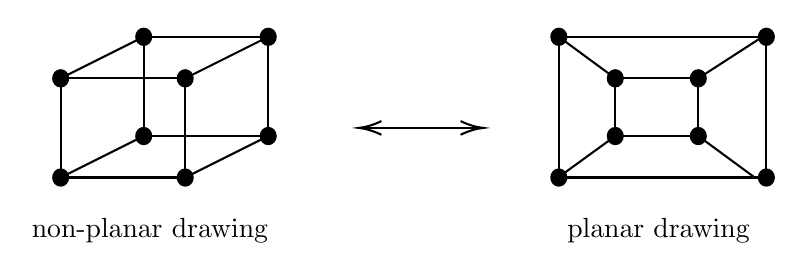
\begin{tikzpicture}[x=0.75pt,y=0.75pt,yscale=-1,xscale=1]
        %uncomment if require: \path (0,300); %set diagram left start at 0, and has height of 300

        %Flowchart: Connector [id:dp8888479749474718] 
        \draw  [fill={rgb, 255:red, 0; green, 0; blue, 0 }  ,fill opacity=1 ] (212.8,36.1) .. controls (212.8,33.95) and (214.41,32.2) .. (216.4,32.2) .. controls (218.39,32.2) and (220,33.95) .. (220,36.1) .. controls (220,38.25) and (218.39,40) .. (216.4,40) .. controls (214.41,40) and (212.8,38.25) .. (212.8,36.1) -- cycle ;
        %Flowchart: Connector [id:dp17636321608858208] 
        \draw  [fill={rgb, 255:red, 0; green, 0; blue, 0 }  ,fill opacity=1 ] (212.8,83.9) .. controls (212.8,81.75) and (214.41,80) .. (216.4,80) .. controls (218.39,80) and (220,81.75) .. (220,83.9) .. controls (220,86.05) and (218.39,87.8) .. (216.4,87.8) .. controls (214.41,87.8) and (212.8,86.05) .. (212.8,83.9) -- cycle ;
        %Flowchart: Connector [id:dp3817279437304819] 
        \draw  [fill={rgb, 255:red, 0; green, 0; blue, 0 }  ,fill opacity=1 ] (272.8,36.1) .. controls (272.8,33.95) and (274.41,32.2) .. (276.4,32.2) .. controls (278.39,32.2) and (280,33.95) .. (280,36.1) .. controls (280,38.25) and (278.39,40) .. (276.4,40) .. controls (274.41,40) and (272.8,38.25) .. (272.8,36.1) -- cycle ;
        %Flowchart: Connector [id:dp5066539288211677] 
        \draw  [fill={rgb, 255:red, 0; green, 0; blue, 0 }  ,fill opacity=1 ] (272.8,83.9) .. controls (272.8,81.75) and (274.41,80) .. (276.4,80) .. controls (278.39,80) and (280,81.75) .. (280,83.9) .. controls (280,86.05) and (278.39,87.8) .. (276.4,87.8) .. controls (274.41,87.8) and (272.8,86.05) .. (272.8,83.9) -- cycle ;
        %Flowchart: Connector [id:dp6775866687809511] 
        \draw  [fill={rgb, 255:red, 0; green, 0; blue, 0 }  ,fill opacity=1 ] (172.8,103.9) .. controls (172.8,101.75) and (174.41,100) .. (176.4,100) .. controls (178.39,100) and (180,101.75) .. (180,103.9) .. controls (180,106.05) and (178.39,107.8) .. (176.4,107.8) .. controls (174.41,107.8) and (172.8,106.05) .. (172.8,103.9) -- cycle ;
        %Flowchart: Connector [id:dp4490381137588745] 
        \draw  [fill={rgb, 255:red, 0; green, 0; blue, 0 }  ,fill opacity=1 ] (232.8,103.9) .. controls (232.8,101.75) and (234.41,100) .. (236.4,100) .. controls (238.39,100) and (240,101.75) .. (240,103.9) .. controls (240,106.05) and (238.39,107.8) .. (236.4,107.8) .. controls (234.41,107.8) and (232.8,106.05) .. (232.8,103.9) -- cycle ;
        %Flowchart: Connector [id:dp9123289761962778] 
        \draw  [fill={rgb, 255:red, 0; green, 0; blue, 0 }  ,fill opacity=1 ] (232.8,56.1) .. controls (232.8,53.95) and (234.41,52.2) .. (236.4,52.2) .. controls (238.39,52.2) and (240,53.95) .. (240,56.1) .. controls (240,58.25) and (238.39,60) .. (236.4,60) .. controls (234.41,60) and (232.8,58.25) .. (232.8,56.1) -- cycle ;
        %Flowchart: Connector [id:dp9409018640344868] 
        \draw  [fill={rgb, 255:red, 0; green, 0; blue, 0 }  ,fill opacity=1 ] (172.8,56.1) .. controls (172.8,53.95) and (174.41,52.2) .. (176.4,52.2) .. controls (178.39,52.2) and (180,53.95) .. (180,56.1) .. controls (180,58.25) and (178.39,60) .. (176.4,60) .. controls (174.41,60) and (172.8,58.25) .. (172.8,56.1) -- cycle ;
        %Straight Lines [id:da17258414213155115] 
        \draw    (176.4,56.1) -- (176.4,103.9) ;
        %Straight Lines [id:da14318992099782368] 
        \draw    (236.4,56.1) -- (236.4,103.9) ;
        %Straight Lines [id:da7989023532097792] 
        \draw    (276.4,36.1) -- (276.4,83.9) ;
        %Straight Lines [id:da7902234351324204] 
        \draw    (216.4,36.1) -- (216.4,83.9) ;
        %Straight Lines [id:da8236407599987878] 
        \draw    (276.4,36.1) -- (216.4,36.1) ;
        %Straight Lines [id:da5909306370785818] 
        \draw    (276.4,83.9) -- (216.4,83.9) ;
        %Straight Lines [id:da3824024136980544] 
        \draw    (236.4,56.1) -- (176.4,56.1) ;
        %Straight Lines [id:da26261891940628845] 
        \draw    (236.4,103.9) -- (176.4,103.9) ;
        %Straight Lines [id:da1524109214467506] 
        \draw    (276.4,36.1) -- (236.4,56.1) ;
        %Straight Lines [id:da7224382816143121] 
        \draw    (216.4,36.1) -- (176.4,56.1) ;
        %Straight Lines [id:da09898252887866943] 
        \draw    (276.4,83.9) -- (236.4,103.9) ;
        %Straight Lines [id:da8530056437131774] 
        \draw    (216.4,83.9) -- (176.4,103.9) ;
        %Flowchart: Connector [id:dp4789528790843105] 
        \draw  [fill={rgb, 255:red, 0; green, 0; blue, 0 }  ,fill opacity=1 ] (412.8,36.1) .. controls (412.8,33.95) and (414.41,32.2) .. (416.4,32.2) .. controls (418.39,32.2) and (420,33.95) .. (420,36.1) .. controls (420,38.25) and (418.39,40) .. (416.4,40) .. controls (414.41,40) and (412.8,38.25) .. (412.8,36.1) -- cycle ;
        %Flowchart: Connector [id:dp3502055889169684] 
        \draw  [fill={rgb, 255:red, 0; green, 0; blue, 0 }  ,fill opacity=1 ] (512.8,36.1) .. controls (512.8,33.95) and (514.41,32.2) .. (516.4,32.2) .. controls (518.39,32.2) and (520,33.95) .. (520,36.1) .. controls (520,38.25) and (518.39,40) .. (516.4,40) .. controls (514.41,40) and (512.8,38.25) .. (512.8,36.1) -- cycle ;
        %Flowchart: Connector [id:dp2974242141498502] 
        \draw  [fill={rgb, 255:red, 0; green, 0; blue, 0 }  ,fill opacity=1 ] (412.8,103.9) .. controls (412.8,101.75) and (414.41,100) .. (416.4,100) .. controls (418.39,100) and (420,101.75) .. (420,103.9) .. controls (420,106.05) and (418.39,107.8) .. (416.4,107.8) .. controls (414.41,107.8) and (412.8,106.05) .. (412.8,103.9) -- cycle ;
        %Flowchart: Connector [id:dp009504262126816987] 
        \draw  [fill={rgb, 255:red, 0; green, 0; blue, 0 }  ,fill opacity=1 ] (512.8,103.9) .. controls (512.8,101.75) and (514.41,100) .. (516.4,100) .. controls (518.39,100) and (520,101.75) .. (520,103.9) .. controls (520,106.05) and (518.39,107.8) .. (516.4,107.8) .. controls (514.41,107.8) and (512.8,106.05) .. (512.8,103.9) -- cycle ;
        %Flowchart: Connector [id:dp06660329132487286] 
        \draw  [fill={rgb, 255:red, 0; green, 0; blue, 0 }  ,fill opacity=1 ] (440,56.1) .. controls (440,53.95) and (441.61,52.2) .. (443.6,52.2) .. controls (445.59,52.2) and (447.2,53.95) .. (447.2,56.1) .. controls (447.2,58.25) and (445.59,60) .. (443.6,60) .. controls (441.61,60) and (440,58.25) .. (440,56.1) -- cycle ;
        %Flowchart: Connector [id:dp36418092614065] 
        \draw  [fill={rgb, 255:red, 0; green, 0; blue, 0 }  ,fill opacity=1 ] (480,56.1) .. controls (480,53.95) and (481.61,52.2) .. (483.6,52.2) .. controls (485.59,52.2) and (487.2,53.95) .. (487.2,56.1) .. controls (487.2,58.25) and (485.59,60) .. (483.6,60) .. controls (481.61,60) and (480,58.25) .. (480,56.1) -- cycle ;
        %Flowchart: Connector [id:dp5960333551593303] 
        \draw  [fill={rgb, 255:red, 0; green, 0; blue, 0 }  ,fill opacity=1 ] (440,83.9) .. controls (440,81.75) and (441.61,80) .. (443.6,80) .. controls (445.59,80) and (447.2,81.75) .. (447.2,83.9) .. controls (447.2,86.05) and (445.59,87.8) .. (443.6,87.8) .. controls (441.61,87.8) and (440,86.05) .. (440,83.9) -- cycle ;
        %Flowchart: Connector [id:dp5325767358067508] 
        \draw  [fill={rgb, 255:red, 0; green, 0; blue, 0 }  ,fill opacity=1 ] (480,83.9) .. controls (480,81.75) and (481.61,80) .. (483.6,80) .. controls (485.59,80) and (487.2,81.75) .. (487.2,83.9) .. controls (487.2,86.05) and (485.59,87.8) .. (483.6,87.8) .. controls (481.61,87.8) and (480,86.05) .. (480,83.9) -- cycle ;
        %Straight Lines [id:da4342589182688269] 
        \draw    (416.4,34.9) -- (416.4,103.9) ;
        %Straight Lines [id:da716956645665608] 
        \draw    (516.4,34.9) -- (516.4,103.9) ;
        %Straight Lines [id:da6672841571831405] 
        \draw    (516.4,36.1) -- (416.4,36.1) ;
        %Straight Lines [id:da8181056438369776] 
        \draw    (516.4,103.9) -- (416.4,103.9) ;
        %Straight Lines [id:da6713047762531956] 
        \draw    (483.6,56.1) -- (443.6,56.1) ;
        %Straight Lines [id:da8582923451456322] 
        \draw    (480,83.9) -- (440,83.9) ;
        %Straight Lines [id:da675355414655931] 
        \draw    (443.6,83.9) -- (443.6,56.1) ;
        %Straight Lines [id:da5260208757512103] 
        \draw    (483.6,83.9) -- (483.6,56.1) ;
        %Straight Lines [id:da15618492588909783] 
        \draw    (443.6,56.1) -- (416.4,36.1) ;
        %Straight Lines [id:da5423111482974576] 
        \draw    (510.8,103.9) -- (483.6,83.9) ;
        %Straight Lines [id:da9783615894342254] 
        \draw    (483.6,56.1) -- (516.4,34.9) ;
        %Straight Lines [id:da5837388726635423] 
        \draw    (414.4,105.1) -- (443.6,83.9) ;
        %Straight Lines [id:da48018342351582766] 
        \draw    (320,80) -- (378,80) ;
        \draw [shift={(380,80)}, rotate = 180] [color={rgb, 255:red, 0; green, 0; blue, 0 }  ][line width=0.75]    (10.93,-3.29) .. controls (6.95,-1.4) and (3.31,-0.3) .. (0,0) .. controls (3.31,0.3) and (6.95,1.4) .. (10.93,3.29)   ;
        %Straight Lines [id:da13703781181033214] 
        \draw    (380,80) -- (322,80) ;
        \draw [shift={(320,80)}, rotate = 360] [color={rgb, 255:red, 0; green, 0; blue, 0 }  ][line width=0.75]    (10.93,-3.29) .. controls (6.95,-1.4) and (3.31,-0.3) .. (0,0) .. controls (3.31,0.3) and (6.95,1.4) .. (10.93,3.29)   ;

        % Text Node
        \draw (161,122) node [anchor=north west][inner sep=0.75pt]   [align=left] {non-planar drawing};
        % Text Node
        \draw (419,122) node [anchor=north west][inner sep=0.75pt]   [align=left] {planar drawing};


    \end{tikzpicture}

\end{center}

Clearly, the left is a non-planar drawing as there are $ 2 $ crossings
within the graph. However, the $ 3 $-cube can be drawn in a planar way
as seen on the right.


\begin{defbox}
    \begin{definition}
        Informally, a \textbf{\emph{planar drawing}} of a graph $ G=(V,E) $
        is a mapping of the vertices of $ G $ to distinct points in
        $ \mathbb{R}^{2} $, and edges of $ G $ to curves between the appropriate
        pair of vertices in such a way that the edges intersect only at their
        common ends.
    \end{definition}
\end{defbox}

\begin{defbox}
    \begin{definition}
        A graph is \textbf{\emph{planar}} if it has a planar drawing.
    \end{definition}
\end{defbox}

\begin{exbox}
    \begin{example}[Planar]
        $ K_4 $ and the $ 3 $-cube are both planar graphs.
    \end{example}
\end{exbox}
\begin{remark}
    It is \textbf{not} correct to say that $ K_4 $ is \emph{sometimes}
    planar depending on how you draw it. It \textbf{is} correct to say
    that $ K_4 $ is a planar graph because there exists a planar drawing.
\end{remark}

This definition is quite hard to utilize for showing a graph is
\emph{not planar}. In fact, there is no obvious way
to prove there \emph{exists} a graph that is not planar since there exists
`infinitely' many possible ways to draw a graph.

Notice that whether you have a planar drawing, you have \emph{faces}.

\begin{remark}
    Many definitions about graph theory within this course will be informal,
    as defining them with rigour will be time consuming. Formal definitions
    can be found in a course like CO 342 (Introduction to Graph Theory),
    and courses about Topology.
\end{remark}

\begin{defbox}
    \begin{definition}
        Given a drawing of a graph,
        let $ X $ be the set of points of $ \mathbb{R}^2 $ that
        are part of the drawing. Informally, the \textbf{\emph{faces}}
        of the drawing are the `connected regions'
        of $ \mathbb{R}^2\setminus X $.
    \end{definition}
\end{defbox}

\begin{remark}
    A planar drawing of a graph is also called an \textbf{\emph{embedding}}.
\end{remark}


\begin{center}
    \includegraphics{l28}
\end{center}

Each face of a connected planar drawing has a \textbf{\emph{boundary walk}}.
This is a closed walk of the graph that follows the boundary of the face.

The boundary walk for $ f_2 $ is:
\[ (v_3,e_3,v_4,e_4,v_5,e_5,v_6,e_6,v_7,e_7,v_3) \]

\begin{defbox}
    \begin{definition}
        If an edge $ e $ belongs to the boundary walk, of a face $ f $,
        we say that $ e $ is \textbf{\emph{incident}} with $ f $.
    \end{definition}
\end{defbox}

\begin{defbox}
    \begin{definition}
        If two faces have boundary walks that share an edge,
        then they are \textbf{\emph{adjacent}}.
    \end{definition}
\end{defbox}

\begin{defbox}
    \begin{definition}
        The \textbf{\emph{degree}} of a face is the length of its
        boundary walk (the number of edges in the walk counting repetitions
        twice).
    \end{definition}
\end{defbox}

\begin{exbox}
    \begin{example}[Degree]
        In the above graph,
        \begin{itemize}
            \item $ f_1 $ has degree $ 3 $
            \item $ f_2 $ has degree $ 6 $
            \item $ f_3 $ has degree $ 9 $
        \end{itemize}
    \end{example}
\end{exbox}

\textbf{Q}: Do the edges in a planar drawing need to be straight
lines?

\textbf{A}: No. (THEOREM (Fary $ \approx 1950 $). It doesn't matter).

\textbf{Q}: What about other surfaces than the plane?

\textbf{A}:
\begin{itemize}
    \item $ \mathbb{R}^3 $? Too easy.
    \item Sphere? Interesting.
    \item Torus?
\end{itemize}

\begin{thmbox}
    \begin{prop}
        The graphs that can be drawn on a sphere (without crossings)
        are just the planar graphs. That is, $ G $ can be drawn
        on a sphere (without crossings)
        if and only if $ G $ can be drawn on the plane.
    \end{prop}
\end{thmbox}

Sketch of \emph{proof}:

$ (\impliedby) $ Obviously true. Planar drawing implies spherical drawing.

$ (\implies) $ Take a hole of a balloon, and stretch it (provided the balloon
does not burst). Eventually, it will end up as a flat surface.

\section{Stereographic Projection}
Think about a sphere on a flat surface. Shine the light source onto the sphere
and a shadow will be casted onto the flat surface.

A 'light source' at $ (0,0,1) $ casts a 'shadow' of the graph on the sphere as
a graph on the plane.

\textbf{Q}: Which graphs can we draw on the torus?

\textbf{A}:
\begin{itemize}
    \item $ K_5 $ is an example of a graph that can be drawn on
          a torus, but cannot be drawn on a plane.
    \item $ K_6 $?
    \item $ K_7 $?
\end{itemize}
